%!TEX root = ../document.tex
\chapter{绪论}
\section{研究背景与意义}

我国经过二十余年的信息化建设,互联网用户仍在持续增长,根据中国互联网信息中心发布的第43次《中国互联网络发展%
状况统计报告》\upcite{43CNNIC}显示,截止2018年12月,我国网民规模达8.29亿,较2017年末仍增加了3.8\%,互联%
网普及率达59.6\%,其中移动互联网用户比例更是高达98.6\%。
浩如烟海的数据填充着互联网,人们要从海量数据中找到自己关心的部分变得越来越难。
推荐系统是帮助用户从海量产品集合里面找到感兴趣目标的软件应用,具有千人千面的特点,也是数据挖掘和机器学习%
相关科技在实践领域最成功的应用之一。
在许多网站和应用程序中,例如电子商务、新闻和视频网站、%
音乐和广播电台等,他们都需要为用户推荐可能喜欢物品的杰出服务,如今接收不同形式的自动推荐已经成为我们日常%
在线用户体验的一部分。在典型的在线网站上面,可以收集用户各种类型的相关动作,例如:用户点击、浏览、收藏、购买%
了某个商品。
推荐系统(RS)已发展成为帮助用户做出明智决策和选择的基本工具,尤其是在大数据时代,%
客户必须从大量产品和服务中做出选择。因此现代推荐系统是在当前大数据环境下应运而生的,%
现代推荐系统的架构如图\ref{fig:RS_Architecture}所示,本文讨论的问题主要出于推荐算法层面。

\begin{figure}[htb]
  \centering
  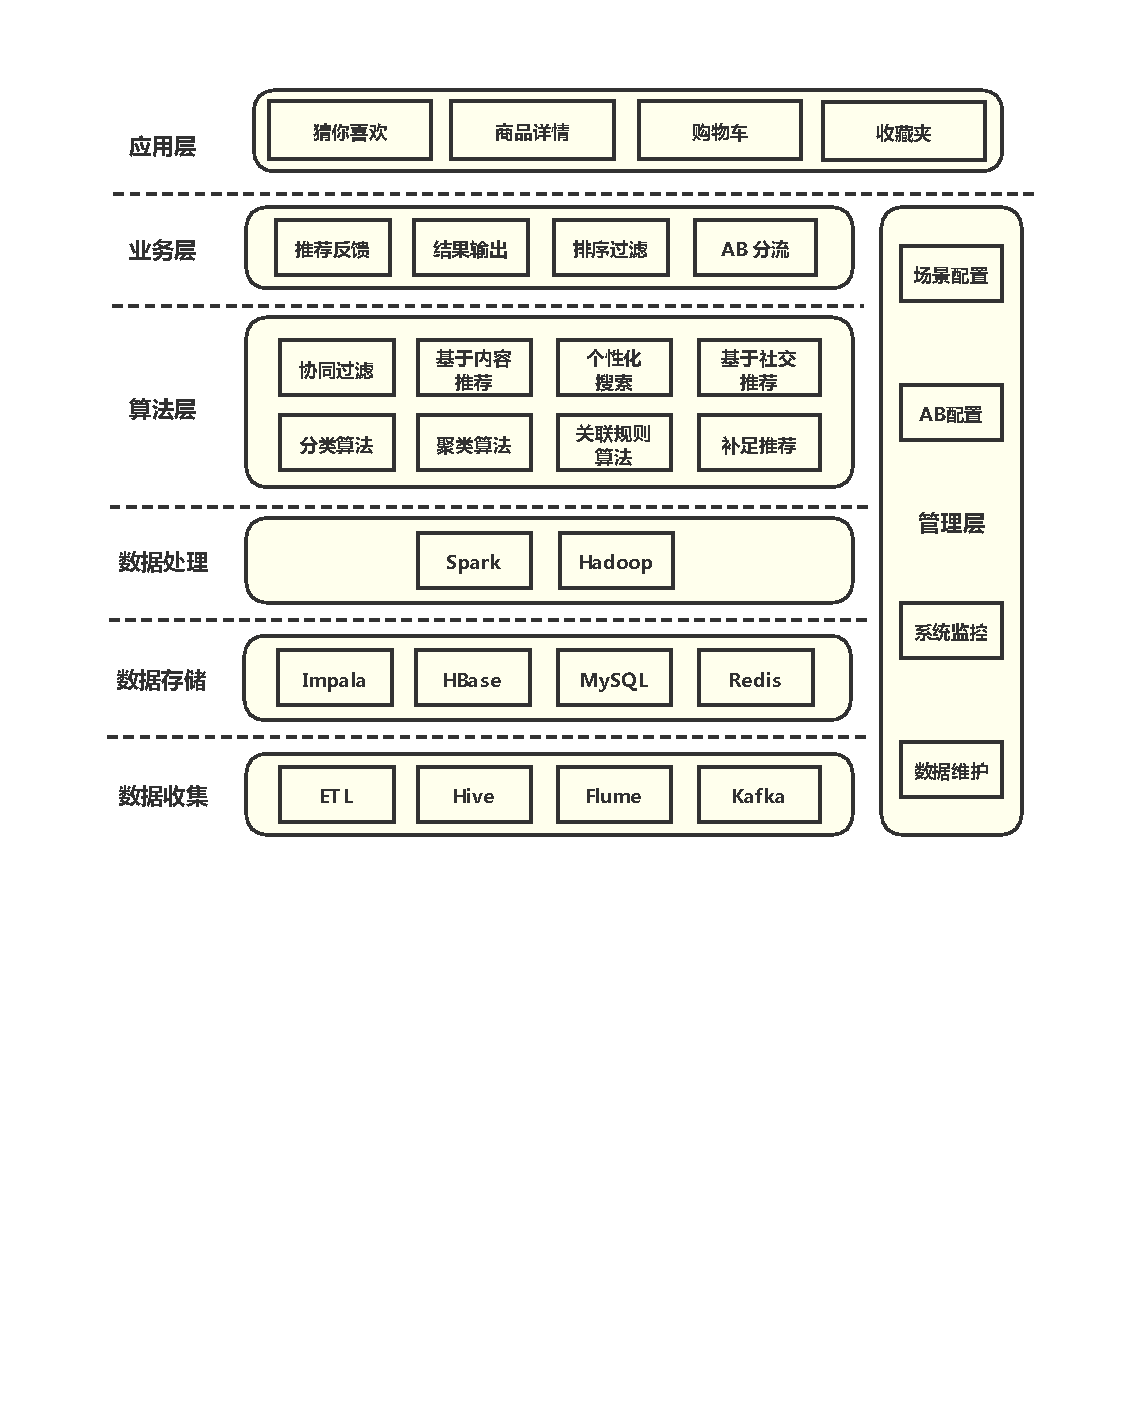
\includegraphics[width=\linewidth]{RS_Architecture.pdf}\\
  \caption{现代推荐系统架构图}
  \label{fig:RS_Architecture}
\end{figure}
推荐算法作为推荐系统的灵魂,承担着推荐高品质项目和高效反馈的重任,因此设计鲁棒性好的推荐算法有着重要的研究意义。
现有的推荐策略都主要关注如何为用户或项目找到临近集,或者利用其它的显式或隐式信息(如标签、评论、%
项目属性和用户个人信息)来提升近邻感知能力。然而,这些静态算法都没有考虑用户兴趣变化的实时动态性。时序信息%
就是反应用户兴趣实时变化的一个重要特征,在许多任务比如用户下一行为预测中,用户下一首会听什么歌与用户的%
喜好、当前所处环境的上下文都高度相关。

推荐系统面对的任务主要有两部分:评分预测和产品推荐。所以根据用户的历史%
记录预测他下一次会选择什么也是推荐领域一个严峻的挑战。

% 推荐系统面临的另外一个巨大挑战就是处理新用户和新物品,也就是所谓的冷启动问题,因为这些用户/物品的特征在缺少数据时很难正确判断。近来,迁移学习\upcite{YangTransfer}被用于解决推荐系统的冷启动问题。迁移学习通过利用辅助域来在目标域上获得提升



本文的研究内容是结合神经网络的序列模型和推荐系统相关理论知识,实现快速向用户推荐可能感兴趣的物品。%
充分利用深度神经网络强大的建模能力,提取用户行为的重要时序特征,构建推荐对象的兴趣模型,%
% 再结合迁移学习的泛化能力,
构建相关模型来识别用户的兴趣意图,综合考虑推荐对象和用户两者之间%
的特征信息挖掘两者之间的隐式联系,从而发掘出用户感兴趣的物品,
以此来帮助用户快速的找到有感兴趣的物品,提升网络应用的流量及用户的黏性。%



2018年的ACM RecSys中还专门设立了关于序列感知推荐的课程并发布了一篇关于序列感知推荐的研究综述\upcite{Quadrana:2018:SRS:3209219.3209270}.



%
本章节主要从传统机器学习和深度学习两个方面介绍现代推荐系统中常用的各种推荐算法,%
从它们各自的特点分析现如今存在的问题。

\section{国内外研究现状}

为了分析和理解国内外现有推荐算法的各自特点,本章节根据其使用的技术不同分为两个大类分别进行描述,
同时给出了如图\ref{fig:RA_clsssification}的思维导图。

\begin{figure}[htb]
  \centering
  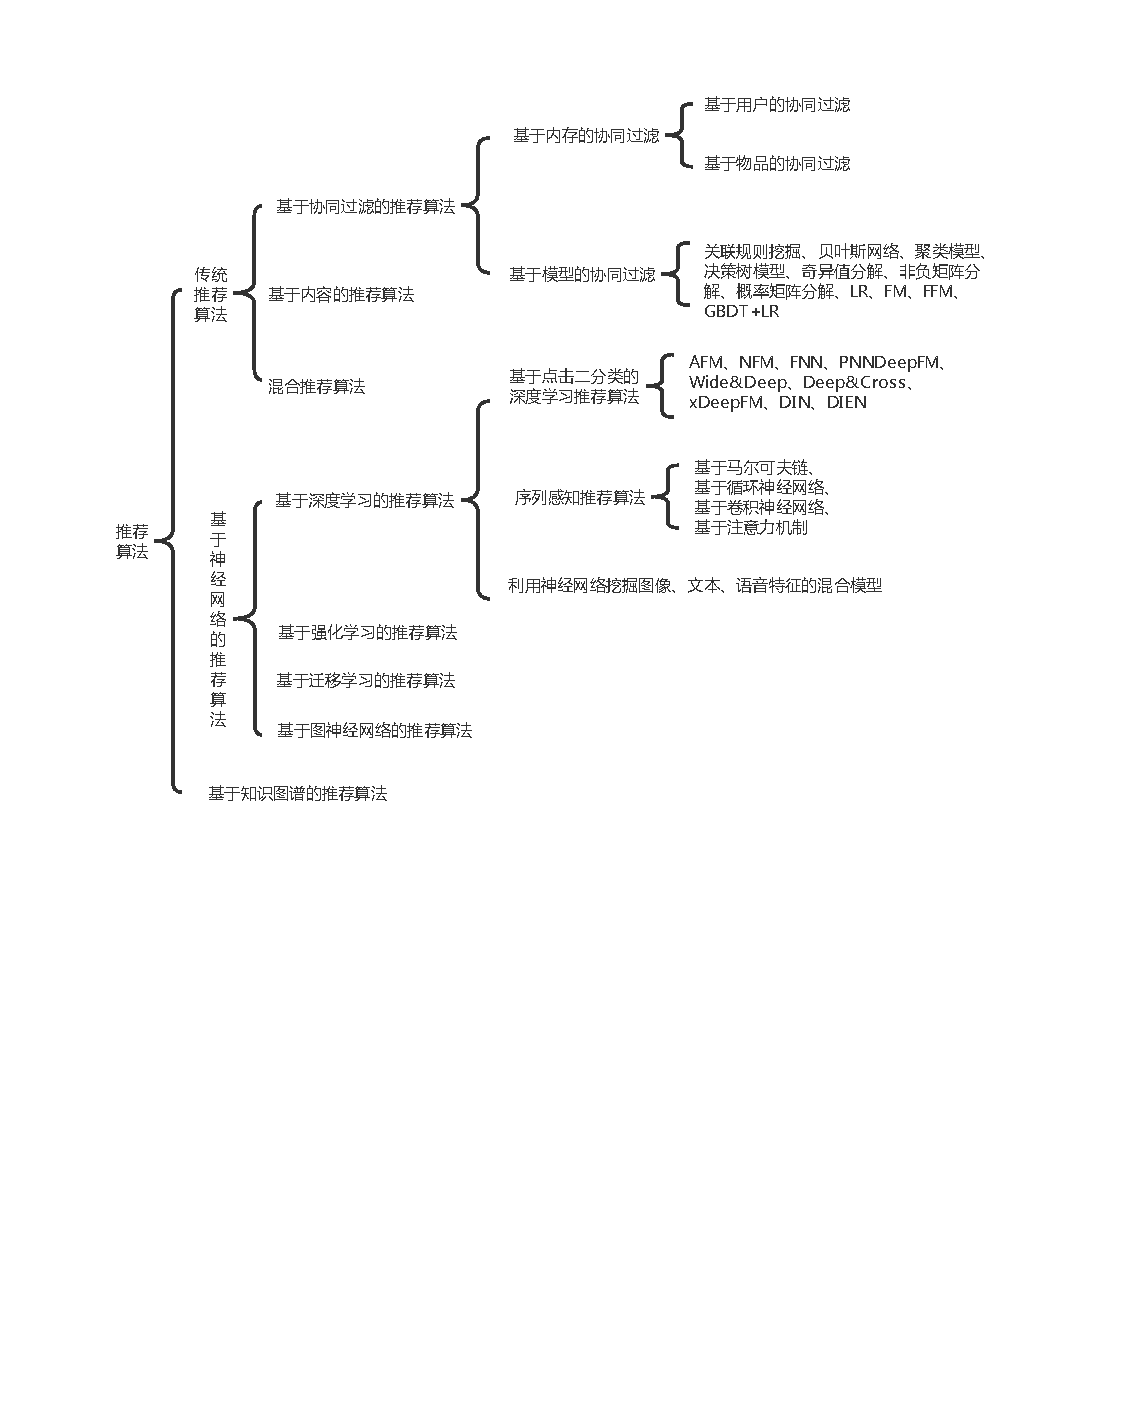
\includegraphics[width=\linewidth]{RA_clsssification.pdf}\\
  \caption{推荐算法分类思维导图}
  \label{fig:RA_clsssification}
\end{figure}

\subsection{传统推荐算法}

传统的经典推荐算法主要可分为三大类,它们分别是基于协同过滤的推荐算法、基于内容的%
推荐算法和混合推荐算法。协同过滤算法大体上可以分为基于内存的协同过滤(Memory-based CF)%
和基于模型的协同过滤(Model-based CF)。基于内存的协同过滤通过为用户寻找具有相似行为的用户%
或有相似特点的物品集合做推荐,所以可细分为基于用户的协同过滤%
(User-based Collaborative Filtering,UBCF)和基于物品的协同过滤%
(Item-based Collaborative Filtering,IBCF)。
而基于模型的协同过滤则主要利用评分信息训练相应的模型,然后使用这个模型对未知数据进行预测,%
这类算法有贝叶斯网络\upcite{Chen02abayesian}、聚类模型\upcite{ungar1998clustering}、%
概率矩阵分解\upcite{NIPS2007_3208}等等。
在基于内容的推荐算法中仅利用了单个用户的行为和数据给出对用户的推荐,特别是物品的描述和用户的属性描述在内容推荐中起到了关键作用。基于内容的
推荐精确度往往有限,还面临着严重的冷启动问题。
混合推荐系统则通过将上述两大类算法中的一个或多个结合起来以避免和克服某个单一算法带来的缺点。混合推荐算法中比较常见的方式是将基于内容的推荐方法与其他方法进行融合以避免冷启动、数据稀疏和扩展性等问题。
基于传统推荐算法的特点,%
基于协同过滤的推荐算法中大多需要构造一个用户与物品的交互矩阵,随着大数据的极速发展,%
物品与用户的数量往往能达到上亿规模,使得交互矩阵构造的空间复杂度过高,在大数据时代传统推荐算法已慢慢无法解决当%
前所面对的问题。

\subsection{基于深度学习的推荐算法}

得益于神经网络的反向传播理论,批量梯度下降的网络权重优化方式使得机器学习特别是深度学习%
能处理的数据规模没有理论上的数量限制,现代推荐算法也借助神经网络的技术蓬勃发展。%
神经网络领域下面子领域里的许多技术都已经被应用于推荐系统当中,包括深度学习、强化学习、迁移学习和图神经网络。%
本文仅讨论基于深度学习的推荐算法。

学术界推荐算法的发展离不开工业界的实践,而推荐算法在工业界的实践应用也为学术界的发展指引着方向。
推荐算法在工业界的一个



% \subsection{个性化推荐研究现状}
\subsection{序列感知推荐研究现状}
% \subsection{迁移学习研究现状}


\section{研究内容和方法}
\subsection{研究内容}
本文通过调研分析科研社交网络的发展状况后,分析了目前科研社交网络在国内外理论和实际应用的情况,%
本文提出一种新的思路去解决学者推荐模型,详细阐述了该学者推荐模型的工作步骤和方式,%
受文本特征提取之关键词抽取的启发,本文还提出了结果评价的指标。最后本文通过爬取“微软学术”官网的%
真实数据对提出的推荐模型的有效性进行验证。本文总体分为六个章节,具体每章的内容安排如下所示:

\subsection{研究方法}
本文主要采用的研究方法有如下几点:
第一,文献调研法。通过互联网技术访问线上各个数据库中检索了大量研究领域的相关书籍、论文等学术成果%
,经过对国内外的相关研究文献与资料的全方位收集和分析,确立本文研究方向和主题,%
设计本文推荐模型框架及各模块之间的耦合。
第二,迁移法,本文是建立在自然语言处理、文本挖掘、推荐系统等相关技术的研究基础之上,通过综合%
探索以上技术理论,将其迁移到本文的模型框架及设计的评价指标上。
第三,实验仿真与分析法,本文通过调研和分析大量文献,提出本文的研究内容,为了验证本文提出的模型的%
有效性,本文在多个真实的数据上进行了实验,从而检验模型的可靠性。

\section{本文主要贡献}
本文通过前期大量文献调研,对比国内外科研社交网站在学者推荐技术上进行的研究,通过深入探索后提出了本文的%
研究问题,并针对提出的问题进行了大规模的对比实验,直到得出最后的结论。整个过程中本文的主要贡献体现%
出如下几点:
\begin{enumerate}
    \item 本文提出了一个基于关键词网络的学者推荐模型,%
          该模型能够根据新用户搜索的关键词进行及时推荐。%
          该模型包含两个网络图,即关键词共现图(Keywords Co-occurrence Graph),%
          为了描述方便,本文简称该图为$KCG$,$KCG$是根据用户学者检索的关键词和匹配到的文献的关键词%
          共同构建的,其目的有二,第一是在用户学者没有明确的意图的情况下,通过挖掘$KCG$中的核心点作为%
          用户学者的搜索意图,第二是通过该图确立用户学者的研究兴趣。另外一个是
          论文学者(Author)和关键词(Keyword)构建的二部图(Graph),简称为$AKG$,该图的目的是%
          采用某种算法对论文学者进行打分排序,以关键词为纽带,建立论文学者和用户学者之间的映射关系,%
          从而向用户学者推荐最有可能感兴趣的论文学者。本文设计的推荐模型通过耦合并挖掘$KCG$和$AKG$两个网络图,%
          最后完成最终的推荐目标。
    \item 本文设计多层过滤器从每篇摘要中抽取关键词集,%
          抽取出的关键词即为论文学者的研究领域或者兴趣。多层过滤器包括采用自然语言处理相关的Pos-Tag标注词性、%
          过滤停用词、正则匹配等启发式的算法过滤生成关键词候选集,还包括文本特征提取中的多个经典%
          特征算法对候选集做进一步过滤,最后采用聚合排序算法对候%
          选关键词集进行重排序,从而生成高质量的关键词集。%
    \item 在学者推荐领域,本文提出了全新的假设,即以关键词网络作为切入点,完成推荐任务。%
          该假设是在缺乏其他指标,如行为记录、基本信息和论文引用数、影响因子等特征,%
          仅仅只使用关键词这一个特征的条件下,设计出了本文的学者推荐模型,该模型能有效解决推荐系统%
          的冷启动问题。为了验证有效性,本文爬取了微软学术官网的文献数据,在真实的数据上验证了模型的可行性。

\end{enumerate}


\section{论文组织架构}

